\documentclass{article}
\usepackage[T1]{fontenc}
\usepackage{hyperref, amssymb, amsmath, graphicx}

\setlength{\oddsidemargin}{.25in}
\setlength{\evensidemargin}{.25in}
\setlength{\textwidth}{6in}
\setlength{\topmargin}{-0.4in}
\setlength{\textheight}{8.5in}

% \setlength{\parindent}{0in}
\setlength{\parskip}{8pt}

\newcommand{\heading}[6]{
	\renewcommand{\thepage}{#1-\arabic{page}}
	\noindent
	\begin{center}
	\framebox{
		\vbox{
			\hbox to 5.78in { \textbf{#2} \hfill #3 }
			\vspace{4mm}
			\hbox to 5.78in { {\Large \hfill #6  \hfill} }
			\vspace{2mm}
			\hbox to 5.78in { \textit{Instructor: #4 \hfill #5} }
		}
	}
	\end{center}
	\vspace*{4mm}
}

\newtheorem{theorem}{Theorem}
\newtheorem{definition}[theorem]{Definition}
\newtheorem{remark}[theorem]{Remark}
\newtheorem{lemma}[theorem]{Lemma}
\newtheorem{corollary}[theorem]{Corollary}
\newtheorem{proposition}[theorem]{Proposition}
\newtheorem{claim}[theorem]{Claim}
\newtheorem{observation}[theorem]{Observation}
\newtheorem{fact}[theorem]{Fact}
\newtheorem{assumption}[theorem]{Assumption}

\newenvironment{proof}{\noindent{\bf Proof:} \hspace*{1mm}}{
	\hspace*{\fill} $\Box$ }
\newenvironment{proof_of}[1]{\noindent {\bf Proof of #1:}
	\hspace*{1mm}}{\hspace*{\fill} $\Box$ }
\newenvironment{proof_claim}{\begin{quotation} \noindent}{
	\hspace*{\fill} $\diamond$ \end{quotation}}
	
\newcommand{\lecture}[4]{\heading{#1}{ECE4880J: Computer Vision}{#2}{Siheng Chen}{#4}{#3}}



%%%%%%%%%%%%%%%%%%%%%%%%%%%%%%%%%%%%%%%%%%%%%%%%%%%%%%%%%%%%%%%%%%%%%%%%%%%%%%%
% PLEASE MODIFY THESE FIELDS AS APPROPRIATE:
\newcommand{\lecturenum}{X} % lecture number
\newcommand{\lecturedate}{June 15, 2022} % date of lecture (e.g., 'March 20, 2010')
\newcommand{\lecturetitle}{Homework 3: Image Processing} % lecture title
\newcommand{\scribename}{{\bf Yiwen Yang}} % full name of scribe
% PUT HERE ANY PACKAGES, MACROS, etc., ADDED BY YOU
%
%%%%%%%%%%%%%%%%%%%%%%%%%%%%%%%%%%%%%%%%%%%%%%%%%%%%%%%%%%%%%%%%%%%%%%%%%%%%%%%
\usepackage{hyperref}
\usepackage[section]{placeins}
\usepackage{caption}
\usepackage{subcaption}
\usepackage{indentfirst}

%%%%%%%%%%%%%%%%%%%%%%%%%%%%%%%%%%%%%%%%%%%%%%%%%%%%%%%%%%%%%%%%%%%%%%%%%%%%%%%
\begin{document}
\lecture{\lecturenum}{\lecturedate}{\lecturetitle}{\scribename}


\section*{Instruction}

\begin{itemize}
	\item This homework is due at 11:59:59 p.m. on ** June 13th, 2022.
	\item The write-up must be a soft copy \texttt{.pdf} file edited by \LaTeX.
	\item The overall submission should be a \texttt{.zip} file named by xxx(student id)-xxx(name)-Assignment3.zip
\end{itemize}


{\bf Python Environment.} We are using \href{https://docs.python.org/3.7/library/index.html}{Python 3.7} for this course. We will use the following packages in this course:
\href{https://numpy.org/}{Numpy},
\href{https://pypi.org/project/opencv-python/}{OpenCV-python},
\href{http://matplotlib.org/users/pyplot tutorial.html}{Matplotlib},
\href{https://pytorch.org/}{Pytorch}.

\section*{Q1. Image Compression}

	\begin{figure}[htb!]
		\centering
		\begin{subfigure}[t]{0.25\textwidth}
			\centering
			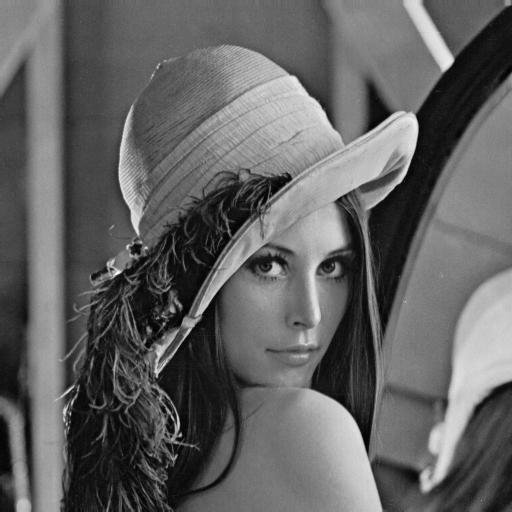
\includegraphics[width=\textwidth]{img/lena_recover.jpg}
			\caption{\label{fig:lena-recover}Recovered globally}
		\end{subfigure}
		\hspace{10em}
		\begin{subfigure}[t]{0.25\textwidth}
			\centering
			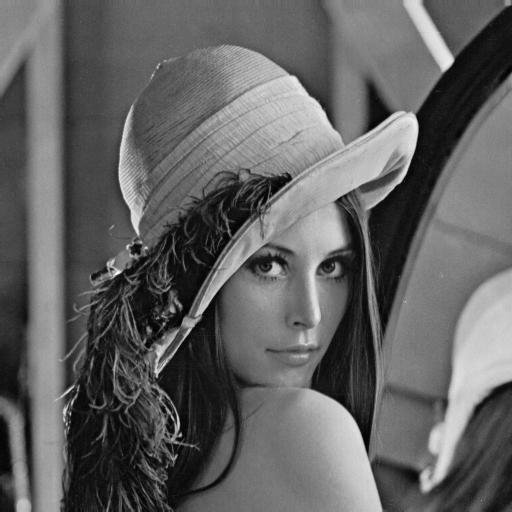
\includegraphics[width=\textwidth]{img/lena_patches_recover.jpg}
			\caption{\label{fig:lena-patch-recover}Recovered in patches}
		\end{subfigure}
		\\
		\begin{subfigure}[t]{0.25\textwidth}
			\centering
			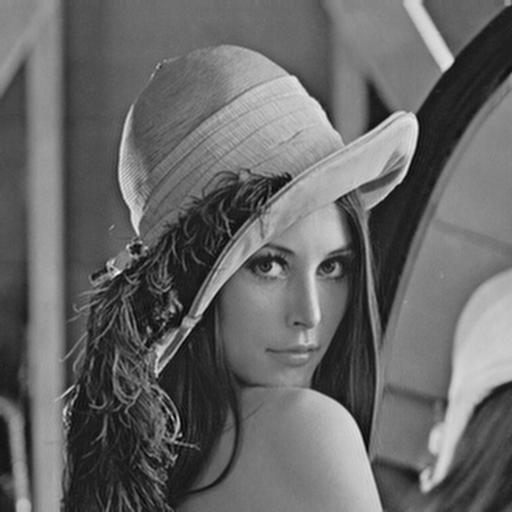
\includegraphics[width=\textwidth]{img/lena_compress_4.jpg}
			\caption{\label{fig:lena-compress-4}Compressed by 1/4}
		\end{subfigure}
		\hfill
		\begin{subfigure}[t]{0.25\textwidth}
			\centering
			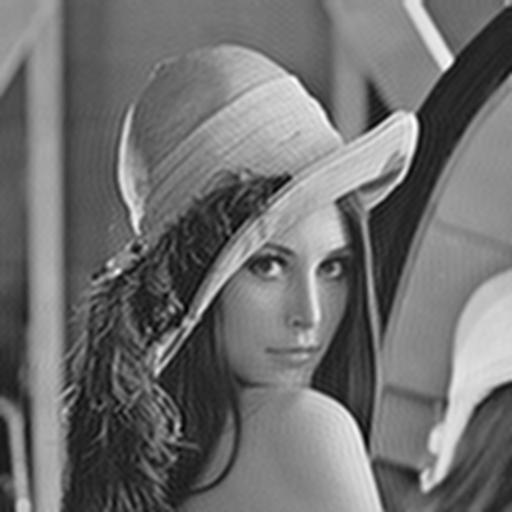
\includegraphics[width=\textwidth]{img/lena_compress_16.jpg}
			\caption{\label{fig:lena-compress-16}Compressed by 1/16}
		\end{subfigure}
		\hfill
		\begin{subfigure}[t]{0.25\textwidth}
			\centering
			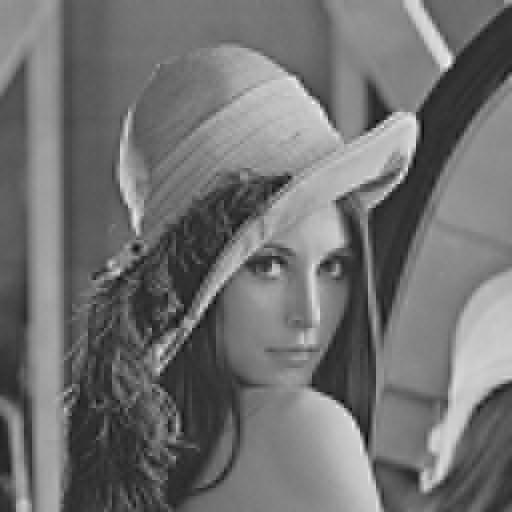
\includegraphics[width=\textwidth]{img/lena_patches_compress.jpg}
			\caption{\label{fig:lena-patch-compress}Compressed by 1/16 in patches}
		\end{subfigure}
		\caption{\label{fig:q1-1}Compression on lena.jpg}
	\end{figure}

	\begin{figure}[htb!]
		\centering
		\begin{subfigure}[t]{0.3\textwidth}
			\centering
			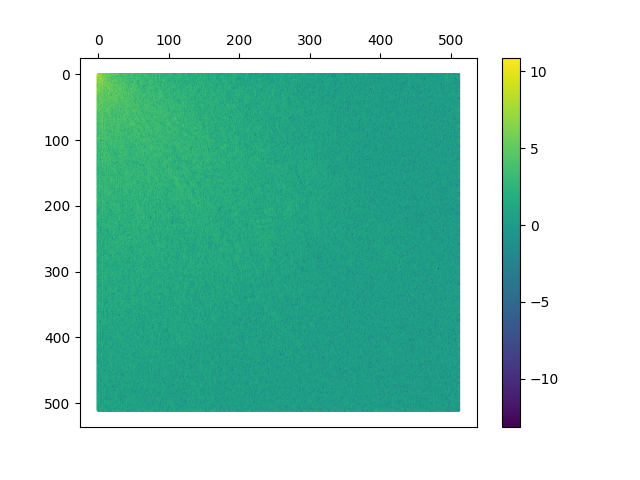
\includegraphics[width=\textwidth]{img/lena_log_map.png}
			\caption{\label{fig:lena-log}Log map of in frequency domain}
		\end{subfigure}
		\begin{subfigure}[t]{0.3\textwidth}
			\centering
			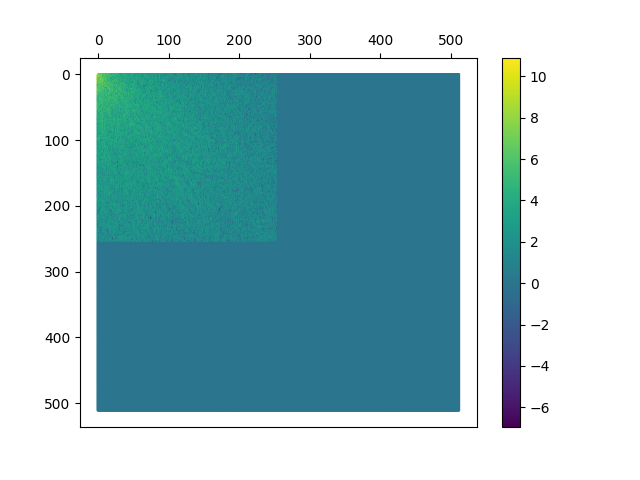
\includegraphics[width=\textwidth]{img/lena_compress_4_log_map.png}
			\caption{\label{fig:lena-log-4}Log map of 1/4 compressed}
		\end{subfigure}
		\hfill
		\begin{subfigure}[t]{0.3\textwidth}
			\centering
			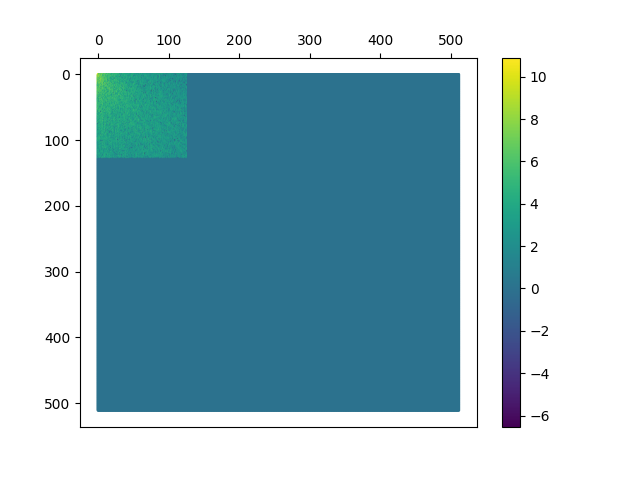
\includegraphics[width=\textwidth]{img/lena_compress_16_log_map.png}
			\caption{\label{fig:lena-log-16}Log map of 1/16 compressed}
		\end{subfigure}
		\hfill
		\caption{\label{fig:q1-2}Log maps}
	\end{figure}

	The recovered images from inverse DCT transformation are exactly the same as the original lena.jpg. Compressing by 1/4 does not seem to change a lot, while compressing by 1/16 is more obvious. Globally compressed images are more continuous, and compression in patches makes the images look dissolved in blocks.

\section*{Q3. Edge Detection}

	\begin{figure}[htb!]
		\centering
		\begin{subfigure}[t]{0.2\textwidth}
			\centering
			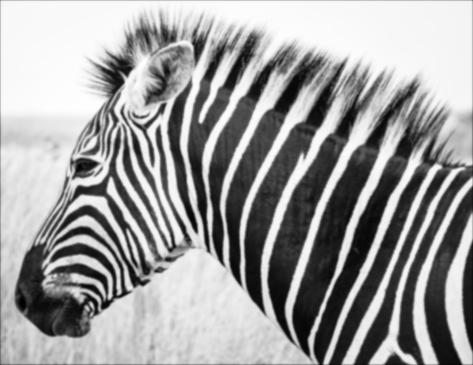
\includegraphics[width=\textwidth]{img/zebra_denoised.jpg}
			\caption{\label{fig:zebra-denoise}Denoise}
		\end{subfigure}
		\hfill
		\begin{subfigure}[t]{0.2\textwidth}
			\centering
			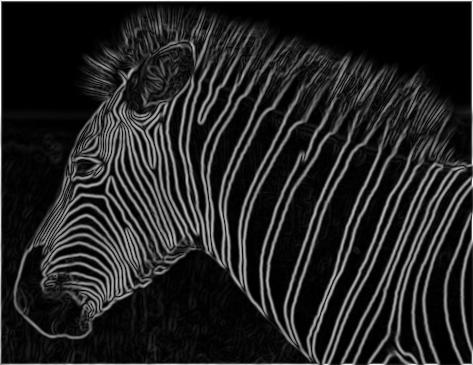
\includegraphics[width=\textwidth]{img/zebra_gradient.jpg}
			\caption{\label{fig:zebra-grad}Intensity gradient}
		\end{subfigure}
		\hfill
		\begin{subfigure}[t]{0.2\textwidth}
			\centering
			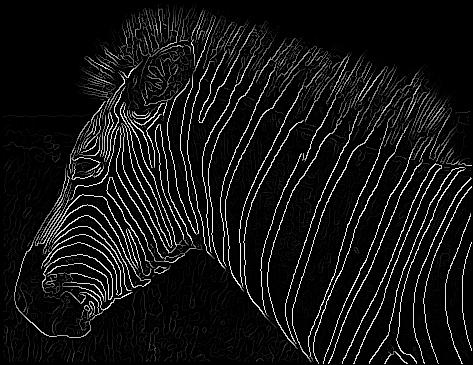
\includegraphics[width=\textwidth]{img/zebra_nms.jpg}
			\caption{\label{fig:zebra-nms}Non-maximum suppression filter}
		\end{subfigure}
		\hfill
		\begin{subfigure}[t]{0.2\textwidth}
			\centering
			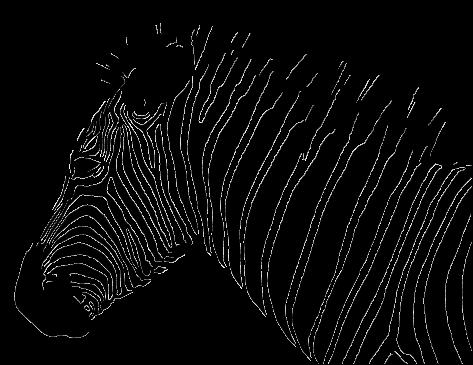
\includegraphics[width=\textwidth]{img/zebra_edge.jpg}
			\caption{\label{fig:zebra-edge}Edges}
		\end{subfigure}
		\caption{\label{fig:q2}Edge Detection of zebra.jpg}
	\end{figure}

	The edges detected are not very perfect. The stripes are correctly figured out, but the back hair is also counted as edges, which is not expected. Even by increasing the threshold, the hair still passes the detection.

\section*{Q4. Line Detection}

	\begin{figure}[htb!]
		\centering
		\begin{subfigure}[t]{0.3\textwidth}
			\centering
			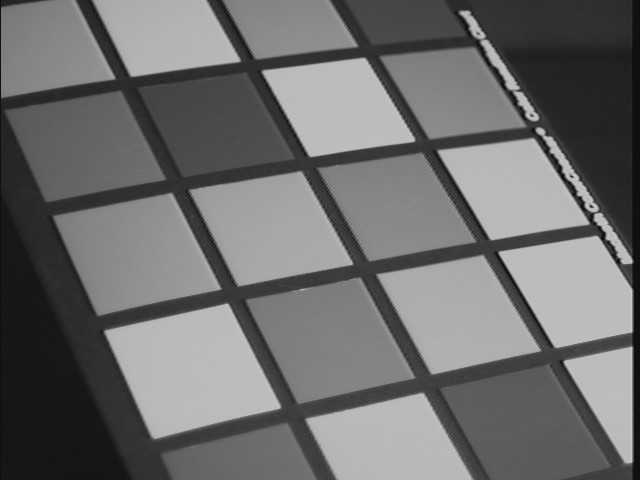
\includegraphics[width=\textwidth]{img/img01.jpg}
			\caption{\label{fig:img-01}img01.jpg}
		\end{subfigure}
		\hfill
		\begin{subfigure}[t]{0.3\textwidth}
			\centering
			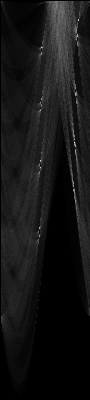
\includegraphics[height=\textwidth]{img/hough01.png}
			\caption{\label{fig:hough-01}Parameter Space}
		\end{subfigure}
		\hfill
		\begin{subfigure}[t]{0.3\textwidth}
			\centering
			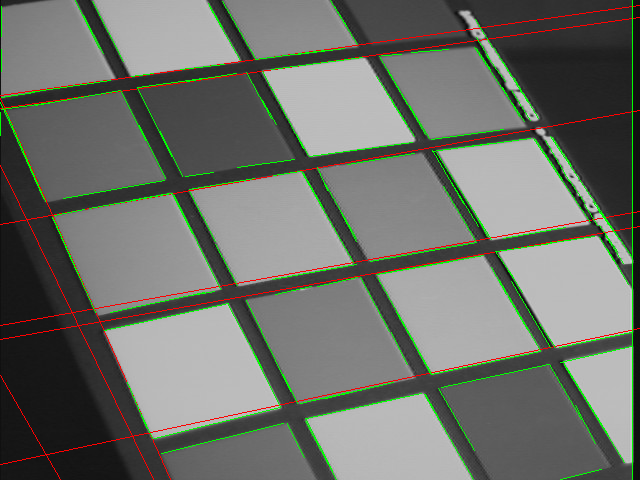
\includegraphics[width=\textwidth]{img/line01.png}
			\caption{\label{fig:line-01}Hough lines}
		\end{subfigure}
		\caption{\label{fig:q3-1}Hough Transform of img01.jpg}
	\end{figure}

	\begin{figure}[htb!]
		\centering
		\begin{subfigure}[t]{0.3\textwidth}
			\centering
			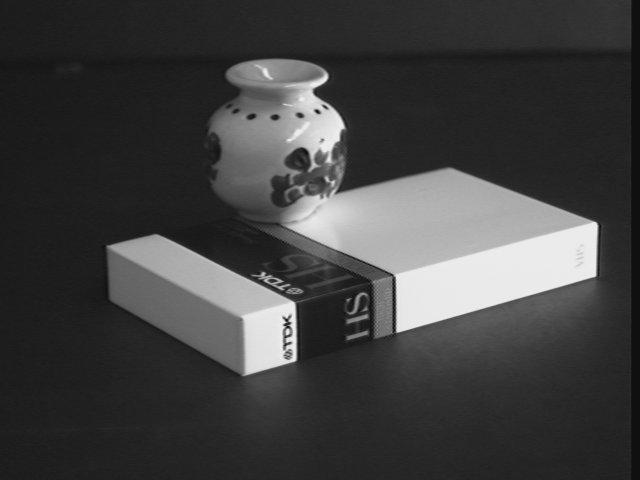
\includegraphics[width=\textwidth]{img/img02.jpg}
			\caption{\label{fig:img-02}img02.jpg}
		\end{subfigure}
		\hfill
		\begin{subfigure}[t]{0.3\textwidth}
			\centering
			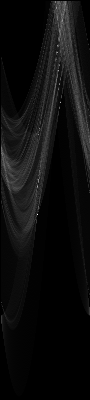
\includegraphics[height=\textwidth]{img/hough02.png}
			\caption{\label{fig:hough-02}Parameter Space}
		\end{subfigure}
		\hfill
		\begin{subfigure}[t]{0.3\textwidth}
			\centering
			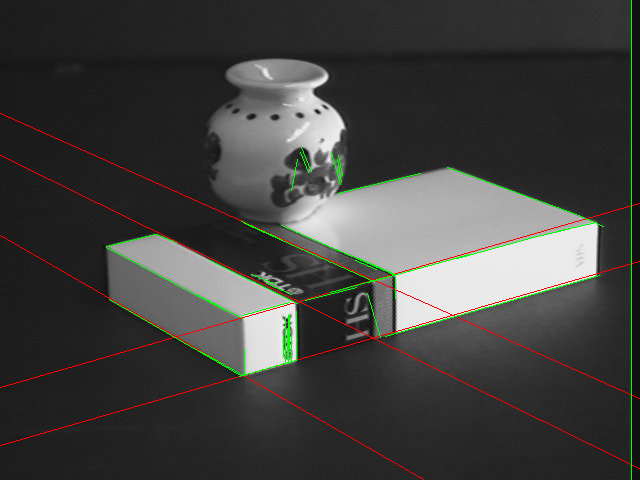
\includegraphics[width=\textwidth]{img/line02.png}
			\caption{\label{fig:line-02}Hough lines}
		\end{subfigure}
		\caption{\label{fig:q3-2}Hough Transform of img02.jpg}
	\end{figure}

	In img01.jpg, 15 lines are detected. Most of the horizontal lines are identified correctly, but only one of the nearly vertical lines was found, which instead can be detected by \texttt{cv2.HoughLinesP()}. There is also one extra line detected at the left-bottom which does not contribute to any real lines, which should be thrown away.

	In img02.jpg, 4 lines are detected. OpenCV appears to detect more lines, and the hand-written one cannot detect more than 4 (all others have very few votes). The top right line (edge of the book) cannot be detected.

\section*{Q5. Feature Extraction}

	\begin{figure}[htb!]
		\centering
		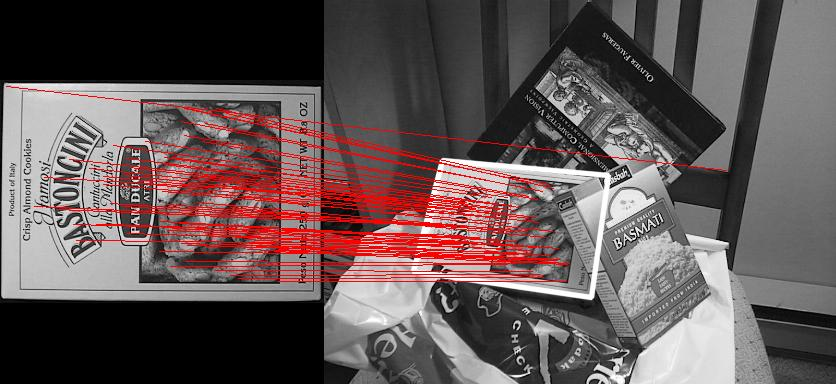
\includegraphics[width=0.5\textwidth]{img/book.jpg}
		\caption{\label{fig:book}SIFT matching of book.jpg}
	\end{figure}

	Most of the features on the book are correctly found and matched. There is one small mismatch that lines up the corner of the book with the corner in the background, which is not expected.

% bibliography goes here
\bibliographystyle{amsalpha}

\end{document}
%%%%%%%%%%%%%%%%%%%%%%%%%%%%%%%%%%%%%%%%%%%%%%%%%%%%%%%%%%%%%%%%%%%%%%%%%%%%%%%